\documentclass{article}

% include graph
\usepackage{graphicx}
% if then else
\usepackage{ifthen}
% for sub itermize
\usepackage{outlines}
% using color package
\usepackage[usenames,dvipsnames]{color}
% 用于产生一种数学用的花体字  
\usepackage{mathrsfs}
% 数学符号  
\usepackage{amsmath,amssymb}
% 专门处理数学粗体的bm宏包
\usepackage{bm}
% 高质量数学字体/黑体  
\usepackage[cmintegrals]{newtxmath}
% Expectation by \E
% just use "\mathbb{E}"
% \DeclareMathOperator{\E}{\mathbb{E}}
% 英文花体, e.g., $\mathcal{D}$
% use table
\usepackage{tabularx}
\usepackage{booktabs}
% use tab
\usepackage{tabto}
% 可以换行的 \underline{}
% \usepackage{ulem} bug: 与emph冲突
% 文字的删除线 \st
\usepackage{soul}
% tickz 画图
\usepackage{tikz}
\usetikzlibrary{graphs}
% for sub figure
\usepackage{subcaption}
% how to write max over x: \max\limits_x

%----------------------------- THE ARTICLE -------------------------------

\begin{document}

\begin{titlepage}
    
\includegraphics[height=3.4cm]{../others/sedes.pdf}
    \\ \\
    \textbf{Machien Learning and Inductive Inference [H02C1a]}
    \\ \\ 
    \textbf{Xinhai Zou (r0727971)}
\end{titlepage}

\pagenumbering{roman} 
\tableofcontents
\clearpage
\pagenumbering{arabic}
\setcounter{page}{1}

\section{Intro to AI}
\subsection{Overview}
AI starts from \textbf{1955} in Bell Telephone Laboratories.
What is AI today?
\begin{outline}
    \1 Planning \& Scheduling
    \1 Declarative Programming
    \1 Robotics
    \1 Computer vision
    \1 Machine learning
    \1 language processing
    \1 Human computer interaction
    \1 theorem proving
\end {outline}
Sometime, we must make a decision when faced with insufficient information.
Being rational means maximizing your expected utility.
\subsection{Summary}
\begin{enumerate}
    \item One summer was not enough to shape AI -> but many significant advances have been made since!
    \item Movie AI, News AI and Research AI differ
    \item Modern AI systems combine 'reasoning' with 'learning' -> this course: 'resoning' focus
    \item Much to say about ethics and fairness of AI systems
\end{enumerate}
\pagebreak
\section{Rational agent}
\subsection{Overview}
\begin{outline}
    \1 Rational agent
        \2 Agent: an entity that perceives (from env.) and acts (to env.)
        \2 Rational: maximizing expected utility
        \2 Rational agent: selects actions that maximize its (expected) utility, i.e., they do the right thing.
    \1 Different environments
        \2 Accessible vs. inaccessible (fully observable vs. partially observable)
            \3 environment is fully observed by agent?
        \2 dterministic vs. stochasitic 
            \3 is the next state of the envioronment completely determined by the current state?
        \2 episodic vs. sequential
            \3 can the quality of an action be evaluated within \textbf{an episode} (perception + action)?
        \2 static vs. dynamic
            \3 can the environment change while the agent is deliberating?
            \3 dynamic - not turn-based game, static - mostly turn-based game
        \2 discrete vs. continuous
            \3 is the value discrete (nominal) or continuous (numerical)
        \2 single vs. multi-agent
            \3 which entities have to regarded as agents? (competitive or cooperative scenarios?)
\end{outline}

Example 
\begin{table}[htbp]\footnotesize
    \centering
    \caption{Examples using different environments}
    \begin{tabularx}{15cm}{X|XXXXXX}
    \toprule
    \textbf{Env.}&\textbf{Observable}&\textbf{Agents}&\textbf{Deterministic}&\textbf{Episodic}&\textbf{Static}&\textbf{Discrete} \\
    \hline
    \textbf{Crossword puzzle}&Fully&Single&Deterministic&\textcolor{red}{sequential}&\textcolor{red}{Static}&Discrete \\
    \hline
    \textbf{Chess with a clock}&&&&&& \\
    \hline
    \textbf{Poker}&&&&&& \\
    \hline
    \textbf{Backgammon}&&&&&& \\
    \hline
    \textbf{Taxi driving}&&&&&& \\
    \hline
    \textbf{Medical diagnosis}&&&&&& \\
    \hline
    \textbf{Image analysis}&&&&&& \\
    \hline
    \textbf{Part-picking robot}&&&&&& \\
    \hline
    \textbf{Refinery controller}&&&&&& \\
    \hline
    \textbf{English tutor}&&&&&& \\
    \hline
    \textbf{Pac-Mac}&Observable&Multi&\textcolor{red}{Stochasitic}&Sequential&\textcolor{red}{Dynamic}&Discrete \\
    \bottomrule
    \end{tabularx}
    \label{tab:diff_classification_association_rules}
\end{table}

\begin{outline}
    \1 Reflex agents
        \2 choose (respond) action only based on current state
        \2 do not consider the future consequences of their actions
    \1 Planning/ Goal based agent
        \2 choose action based on consequences of actions (future)
        \2 consider how the world will be
\end{outline}

\subsection{Summary}
\begin{enumerate}
    \item an agent is something that perceives and acts, being rational is to obtain maximal expected value. An rational agent will take the action that maximizes its expected performance given the percept sequence and its knowledge of the environment.
    \item an agent program maps from a percept to an action
    \begin{enumerate}
        \item reflex agents respond based on current state
        \item goal-based agents respond based on current and future state
        \item learning agents improve their behaviour over time
    \end{enumerate}
    \item some environments are more demanding than others
\end{enumerate}

\pagebreak
\section{State space}
\subsection{Overview}
How to represent a problem in machine? For a basic search problem, there are five ingredients.
\begin{enumerate}
    \item States: represent the states in a clear way
    \item Actions: define the actions you can execute and change the world state, normally $\delta: X \rightarrow Y$
    \item Initial state: what is the initial state, the \textbf{starting} point
    \item Goal formulation: define which states you want to end
    \item Specification of the search cost: the execution costs
\end{enumerate} 

\noindent
Take Pac-man - path-finding as an example, which is shown below:
\begin{outline}
    \1 States: $(x,y)$, where x is x-axis and y is y-axis
    \1 Initial state: starting point $(x_{0},y_{0})$
    \1 Actions: different actions
        \2 east: $f_{east}: (x,y) \rightarrow (x+1,y)$
        \2 west: $f_{west}: (x,y) \rightarrow (x-1,y)$
        \2 north: $f_{north}: (x,y) \rightarrow (x,y+1)$
        \2 south: $f_{south}: (x,y) \rightarrow (x,y-1)$
    \1 Goal test: goal point/state $(x^{*},y^{*})$
    \1 Path cost: each step cost 1 step unit, only have <specific number> state unit
\end{outline}

\noindent
Sometimes, we need a check-loop detection. We have two different structure for state-space representation: graph and search tree.
\begin{outline}
    \1 graph
        \2 For graph, during searching, we often keep track of the already visited nodes to avoid loops and redundancies.
    \1 search tree
        \2 nodes show states, each node in the search tree is an entire PATH in the state space graph.
\end{outline}

\noindent
Some key issues:
\begin{outline}
    \1 definition of state space and transition model
    \1 choose implicit graph or implicit tree
    \1 search forward or backward
    \1 use optimal solution or any solution
    \1 decompose difficult problem to simpler problem (problem reduction/ decomposability)
\end{outline}

\noindent
For forward and backward search, the definition is shown as belwo. The efficiency can be improved based on different branching factor. However, backward is not always possible, e.g., playing chess.
\begin{enumerate}
    \item Forward: start from initial state and search towards goal
    \item Backward: start from the goal state and search toward initial state
\end{enumerate}

\subsection{Summary}
\begin{enumerate}
    \item Before an agent can start to perform on searching problem, 5 ingredients are important:
    \begin{enumerate}
        \item State
        \item Initial state
        \item Goal state
        \item Action
        \item Cost
    \end{enumerate}
\end{enumerate}

\pagebreak
\section{Uniformed search}
\subsection{Overview}
Some terminologies for searching problem in graph:
\begin{enumerate}
    \item node expansion: generating all successor node considering the availble actions (the whole process)
    \item explored nodes: nodes that have already been expanded
    \item frontier/ fringe: set of all nodes available for expansion (candidate for expansion)
    \item search stratege: defines which node is expanded next (the strategies)
\end{enumerate}

\noindent
\subsection{Graph search}
Graph search, frontier = {<s,a>, <s,b>}, its \textcolor{blue}{basic} algorithm: \\
\textbf{Input:} \\
\tabto{5mm} a graph, \\
\tabto{5mm} a set of start nodes, \\
\tabto{5mm} Boolean procedure \emph{goal(n)} that tests if \emph{n} is a goal node. \\
\emph{frontier} := {$<s>$, $s$ is a start node} \\
\textbf{while} \emph{frontier} is not empty: \\
\tabto{5mm} \textbf{select} and \textbf{remove} path $<n_{0},...,n_{k}>$ from \emph{frontier} \textbf{for every} neighbor $n$ of $n_{k}$ \\
\tabto{10mm} \textcolor{blue}{\textbf{if} \emph{goal(n)}} \\
\tabto{15mm} \textcolor{blue}{\textbf{return} $<n_{0},...,n_{k},n>$} \\
\tabto{10mm} \textbf{else add} $<n_{0},...,n_{k},n>$ to \emph{frontier} \\
\textbf{end while} \\

\noindent
For loop detection, the \textcolor{red}{loop-detection} algorithm will be: \\
\textbf{Input:} \\
\tabto{5mm} a graph, \\
\tabto{5mm} a set of start nodes, \\
\tabto{5mm} Boolean procedure \emph{goal(n)} that tests if \emph{n} is a goal node. \\
\emph{frontier} := {$<s>$, $s$ is a start node} \\
\textbf{while} \emph{frontier} is not empty: \\
\tabto{5mm} \textbf{select} and \textbf{remove} path $<n_{0},...,n_{k}>$ from \emph{frontier} \textbf{for every} neighbor $n$ of $n_{k}$ \\
\tabto{10mm} \textcolor{blue}{\textbf{if} \emph{goal(n)}} \\
\tabto{15mm} \textcolor{blue}{\textbf{return} $<n_{0},...,n_{k},n>$} \\
\tabto{10mm} \textcolor{red}{\textbf{else if} $n \notin {n_{0},...,n_{k}}$} \\
\tabto{15mm} \textbf{then add} $<n_{0},...,n_{k},n>$ to \emph{frontier} \\
\textbf{end while} \\

Two basic searching strategies for selecting nodes to explore: depth-first search and breadth-first search.

\subsection{DFS and BFS}
\subsubsection{Depth-First Search (DFS)}
Its selecting strategy is \textbf{LIFO = "Last In First Out"}, we work with \textbf{stack}. 
\begin{outline}
    \1 Time complexity: $O(b^{m})$
        \2 with b: branching factor, m: maximum depth
    \1 Space complexity: $O(b \times m)$
        \2 with b: branching factor, m: maximum depth
\end{outline}

\noindent
The property of DFS:
\begin{outline}
    \1 Time complexity: $O(b^{m})$
    \1 Space complexity: $O(b \times m)$
    \1 Completeness: is complete if finite m and prevent loop
    \1 Optimal: no guarantee, it finds the leftmost solution
\end{outline}

\subsubsection{Breadth-First Search (BFS)}
Its selecting strategy is \textbf{FIFO = "First In First Out"}, we work with \textbf{queue}.
\begin{outline}
    \1 Time complexity: $O(b^{s})$
        \2 with b: branching factor, s: shallowest-solution depth
    \1 Space complexity: $O(b^{s})$
        \2 with b: branching factor, s: shallowest-solution depth
    \1 Completeness: no matter loop or not, it is complete
    \1 Optimal: optimal only if \textbf{cost between each node = 1}
\end{outline}

\subsubsection{Comparison of DFS \& BFS}
DFS uses less memory, but needs loop detection; while BFS use more memory, but does not need loop detection. More details are shown as below: \\
\begin{outline}
    \1 Depth-First Search
        \2 Space is restricted
        \2 Many solutions exist, solutions are long
        \2 no infinite paths
    \1 Breadth-First Search
        \2 Space is not a problem
        \2 Solution containing fewest/shallowest depth
\end{outline}

\subsection{Iterative Deepening}
Iterative Deepening is a combinatino of DFS and BFS, the idea is to get advantages from both DFS (space complexity) and BFS (time complexity, optimal, completeness). Run a DFS with depth limit 0/1/2/3/.... (P.S.:LIFO-stack, FIFO-queue). \\
Furthermore, the \textbf{outter} algorithm: \\
\textbf{procedure iterative-deepening (} \\
\tabto{5mm} \textbf{Input:}  \\
\tabto{5mm} a graph, \\
\tabto{5mm} a set of start nodes, \\
\tabto{5mm} Boolean function \emph{goal(n)} that tests if \emph{n} is a goal mode \\
\textbf{)} \\
\emph{depthlimit = 1} \\
\textbf{while} goal not found \textbf{do} \\
\tabto{5mm} call depth-limited-search(graph, starting nodes, \emph{goal(n)}, \emph{depthlimit})
\tabto{5mm} \emph{depthlimit = depthlimit + 1} \\

\noindent
The \textbf{inner} algorithm: \\
\textbf{procedure depth-limited-search(} \\
\tabto{5mm} \textbf{Input:}  \\
\tabto{5mm} a graph, \\
\tabto{5mm} a set of start nodes, \\
\tabto{5mm} Boolean procedure \emph{goal(n)} that tests if \emph{n} is a goal node, \\
\tabto{5mm} \textcolor{red}{\emph{depthlimit}: natural number} \\
\textbf{)} \\
\emph{frontier} := {$<s>$ : $s$ is a start node} \\
\textbf{while} \emph{frontier} is not empty: \\
\tabto{5mm} \textbf{select} and \textbf{remove} \textcolor{red}{first} path $<n_{0},...,n_{k}>$ from \emph{frontier} \\
\tabto{5mm} \textcolor{red}{\textbf{if} \emph{k < depthlimit}} \\
\tabto{10mm} \textbf{for every} neighbor $n$ for $n_{k}$ \\
\tabto{15mm} \textcolor{blue}{\textbf{if} \emph{goal(n)}} \\
\tabto{20mm} \textcolor{blue}{\textbf{then return $n_{0},...,n_{k},n$}} \\
\tabto{15mm} \textbf{else add} $n_{0},...,n_{k},n$ to \textcolor{red}{start of} \emph{frontier} \\
\textbf{end while} \\

\noindent
The property of iterative deepening (ID) is similar to BFS, the only difference is the memory usage which is better than BFS ($O(b \times s) \ge O(b^{s})$). \emph{Time complexity almost is the same as BFS, the only difference is ID needs iterative reconstruction each limit of 0,1,2,3 needs to start from start node (root) and to rebuild the search tree}
\begin{outline}
    \1 Time complexity: $O(b^{s})$
        \2 with b: branching factor, s: shallowest-solution depth
    \1 Space complexity: $O(b \times s)$
        \2 with b: branching factor, s: shallowest-solution depth
    \1 Completeness: no matter loop or not, it is complete
    \1 Optimal: optimal only if \textbf{cost between each node = 1}
\end{outline}

\subsection{Bi-directional search}
Forward and backward search together. But it is not always possible \emph{because backward is not always known}. The algorithm is shown below: \\
\textbf{Input:} \\
\tabto{5mm} a graph, \\
\tabto{5mm} a set of start nodes, \\
\tabto{5mm} Boolean procedure \emph{goal(n)} that tests if \emph{n} is a goal node. \\
$frontier_{0}$ := {$<s>$: $s$ is a start node} \\
$frontier_{1}$ := {$<g>$: $g$ is a goal node} \\
$i$ := 0; \\
\textbf{while} $frontier_{1}$ and $frontier_{0}$ not empty: \\
\tabto{5mm} $i$ := $i+1$ mode $2$; $j$ := $i+1$ mod $2$; (swap $i$ and $j$) \\
\tabto{5mm} \textbf{select} and \textbf{remove} first path $<n_{0},...,n_{k}>$ from $frontier_{i}$ \\
\tabto{5mm} \textbf{for every} neighbor $n$ of $n_{k}$ in direction $i$ \\
\tabto{10mm} \textbf{if} $n$ occurs in path $<n^{\prime}_{0},...,n^{\prime}_{l}>$ of $frontier_{j}$ with l the length of n in $frontier_{j}$ \\
\tabto{15mm} \textbf{return} solution based on $<n^{\prime}_{0},...,n^{\prime}_{l}>$ and $<n_{0},...,n_{k}>$ \\
\tabto{10mm} \textbf{else add} $<n_{0},...,n_{k},n>$ to end of $frontier_{i}$ \\
\textbf{end while} \\

\noindent
The property of Bi-directional search:
\begin{outline}
    \1 Time complexity: $O($\textcolor{red}{$2 \times$}$b^{\frac{d}{2}})$
        \2 with b: branching factor, d:maximum depth
    \1 Space complexity: $O($\textcolor{red}{$2 \times$}$b^{\frac{d}{2}})$
        \2 with b: branching factor, d:maximum depth
    \1 Completeness: yes
    \1 Optimal: \textcolor{red}{yes} <- \textbf{why?}
\end{outline}

\subsection{Uniform Cost Search (UCS)}
BFS finds the shortest path in terms of number of actions. However, it does not find the least-cost path. We will now consider the cost between 2 nodes. \\
\textbf{The formula: $cost(<n_{0},n_{1},...,n_{k}>) = \sum_{i=1}^{k} cost(<n_{i-1},n_{i}>)$} \\
\textbf{SELECT} becomes \textbf{"priority queue, select element with lowest cost first"} \\
Two possibilities in graph searching: first version and last version.
\begin{enumerate}
    \item First version: after selecting first lowest-cost node, done.
    \item Last version: after checking every lowest-cost node, then done (more optimal).
\end{enumerate}

\noindent
Then we can have a further optimization: \textbf{Branch-and-bound principle:} when a goal is found along a path with cost C, prune all paths on the frontier with cost > C, where these cost can never be optimal since their cost has already > C. \\
The properties of UCS are: \\
The property of Bi-directional search:
\begin{outline}
    \1 Time complexity: $O(b^{1+\frac{C^{*}}{\epsilon}})$
        \2 with b: branching factor, $C^{*}$: solution cost, arc cost (cost between 2 neighbor nodes) at least $\epsilon$
    \1 Space complexity: $O(b^{1+\frac{C^{*}}{\epsilon}})$
        \2 with b: branching factor, $C^{*}$: solution cost, arc cost (cost between 2 neighbor nodes) at least $\epsilon$
    \1 Completeness: yes (minimum arc cost is positive, $\epsilon > 0$)
    \1 Optimal: yes
\end{outline}

Remember: UCS explains increasing \textbf{cost contours}.
\begin{outline}
    \1 Pros:
        \2 Complete and Optimal!
    \1 Cons:
        \2 Explores option in every "direction", just like BFS
        \2 No information about goal location, only accumulation of cost (advanced algorithm should have advanced function/info providing)
\end{outline}

\subsection{Summary}
\begin{enumerate}
    \item The difference between each algorithm: \textbf{which node on the frontier will be explored next}.
    \item Search algorithm is judged by its properties: \textbf{time complexity, space complexity, completeness, optimality}.
\end{enumerate}

\pagebreak
\section{Informal search}
\subsection{Overview}
Different from uninformed search and informed search. 
\begin{outline}
    \1 Uninformed search
        \2 use only information on \textbf{current path}, that is, from goal to fringe
    \1 Informed search
        \2 use also \textbf{heuristics}, that is, information about how close nodes on the fringe are to a goal
\end{outline}

\noindent
A heuristics is a function that estimates \textbf{how close a state is to a goal}, which needs \textbf{domain knowledge} \\

There is different heuristic function: manhattan distance, euclidean distance, ....

\subsection{Greedy search}
The difference between greedy search and uniformed search is \textbf{SELECT = "priority queue, order elements by $h(n)$}, which is called "Best-first search". \\
The difference between greedy search and uniformed cost-sensitive search is:
\begin{outline}
    \1 Greedy Search uses heuristic to order.
    \1 UCS uses accumulated cost to order.
\end{outline}

\noindent
Is it optimal? No, it just takes \textbf{the most obvious result} as next step, but may not be the best one. (Short-term vs. Long-term) Thus, the properties of greedy search is: (Time and space complexity is just badly-guide DFS)
\begin{outline}
    \1 Time complexity: $O(b^{m})$
        \2 with b: branching factor, m: maximum depth
    \1 Space complexity: $O(b^{m})$
        \2 with b: branching factor, m: maximum depth
    \1 Completeness: \textcolor{red}{no}, like badly DFS
    \1 Optimal: \textcolor{red}{no}, it just choose the most obvious result instead of the optimal one
\end{outline}

\subsection{Beam search}
A variant of \st{greedy search} and breadth-first search. It is similar to breadth-first, but only expend \emph{k} times \textbf{each tier}. First build the whole tier, then keep \emph{k} elements in frontier. The properties of beam search is:
\begin{outline}
    \1 Time complexity: \textcolor{red}{$O(k \times b \times s)$}
        \2 with k: hyperparameter, b: branching factor, s: shallowest-solution depth
    \1 Space complexity: \textcolor{red}{$O(k \times b)$}
        \2 with k: hyperparameter, s: shallowest-solution depth
    \1 Completeness: no, may drop the goal
    \1 Optimal: no, not completeness not even optimal
\end{outline}

\noindent
When k = 1, it is called \textbf{"Hill-Climbing search"}. \\

\subsection{Combination of UCS and Greedy Search}
As we known, UCS uses \textbf{path cost = "Backward cost" = $g(n)$} (Figure~\ref{fig:usc_path_cost}), and Greedy search uses \textbf{heuristic = "Forward cost = $h(n)$} (Figure~\ref{fig:greedy_search_heuristic}). And if we combine those two cost to estimate the quality of our current state: $f(n) = g(n) + h(n)$. The \textbf{SELECT = "priority queue, order elements by $f(n)$"} \\

\begin{figure}[htbp]
    \centering
    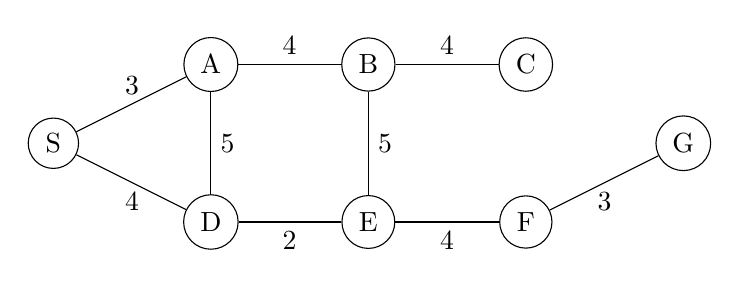
\begin{tikzpicture}
        \node [draw,circle](s)at(0,0){S};
        \node [draw,circle](a)at(2,1){A};
        \node [draw,circle](d)at(2,-1){D};
        \node [draw,circle](b)at(4,1){B};
        \node [draw,circle](e)at(4,-1){E};
        \node [draw,circle](c)at(6,1){C};
        \node [draw,circle](f)at(6,-1){F};
        \node [draw,circle](g)at(8,0){G};

        \draw (s) -- (a); 
        \draw (a) -- (b);
        \draw (b) -- (c);
        \draw (a) -- (d);
        \draw (s) -- (d);
        \draw (d) -- (e);
        \draw (b) -- (e);
        \draw (e) -- (f);
        \draw (f) -- (g);        

        \draw (1,1/2) node[above]{$3$};
        \draw (1,-1/2) node[below]{$4$};
        \draw (2,0) node[right]{$5$};
        \draw (3,1) node[above]{$4$};
        \draw (3,-1) node[below]{$2$};
        \draw (4,0) node[right]{$5$};
        \draw (5,1) node[above]{$4$};
        \draw (5,-1) node[below]{$4$};
        \draw (7,-1/2) node[below]{$3$};
    \end{tikzpicture}
    \caption{Path cost $g(n)$}
    \label{fig:usc_path_cost}
\end{figure}

\begin{figure}[htbp]
    \centering
    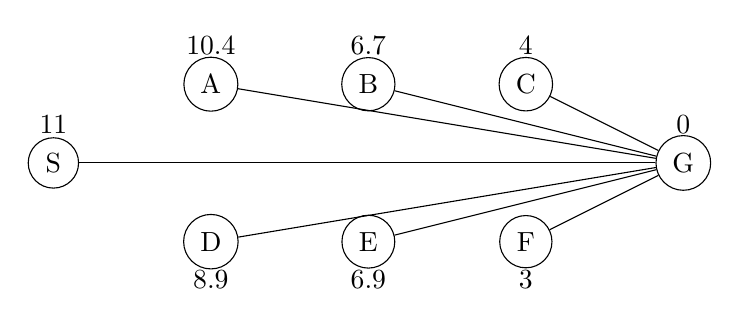
\begin{tikzpicture}
        \node [draw,circle](s)at(0,0){S};
        \node [draw,circle](a)at(2,1){A};
        \node [draw,circle](d)at(2,-1){D};
        \node [draw,circle](b)at(4,1){B};
        \node [draw,circle](e)at(4,-1){E};
        \node [draw,circle](c)at(6,1){C};
        \node [draw,circle](f)at(6,-1){F};
        \node [draw,circle](g)at(8,0){G};

        \draw (s) -- (g);
        \draw (a) -- (g);       
        \draw (d) -- (g);
        \draw (b) -- (g);
        \draw (e) -- (g);
        \draw (c) -- (g);
        \draw (f) -- (g);

        \draw (0,1/4) node[above]{$11$};
        \draw (2,5/4) node[above]{$10.4$};
        \draw (2,-5/4) node[below]{$8.9$};
        \draw (4,5/4) node[above]{$6.7$};
        \draw (4,-5/4) node[below]{$6.9$};
        \draw (6,5/4) node[above]{$4$};
        \draw (6,-5/4) node[below]{$3$};
        \draw (8,1/4) node[above]{$0$};
    \end{tikzpicture}
    \caption{Heuristic $h(n)$}
    \label{fig:greedy_search_heuristic}
\end{figure}

\noindent
However, this is not enough for optimal. We need to do something on the heuristic cost. Otherwises, the actual bad goal cost < estimated good goal cost. \textbf{Admissible heuritics} is needed, they \textbf{underestimate the actual cost}. Saying that $h$ is admissible iff for all nodes $n \le h(n) \le h^{*}(n)$ where $h^{*}(n)$ is the actual cost to the closest goal. \\
How to come up with admissible heuristics? The cost of an optimal solution to a \textbf{relaxed problem} is admissible heuristics, an understimate, for the original problem. \\
Larger admissible heuristics, better estimation, closer to actual value, \textcolor{red}{but cannot larger than actual value (upper bound).} For example, $h2$ dominates $h1$ means for all nodes $n: h2(n) \ge h1(n)$. In this case, $h2$ is always better than $h1$, but for all nodes $h1(n) \le h2(n) \le h^{*}(n)$. For two heuristics $h1$ and $h2$, $h3(n) = max(h1(n),h2(n))$ always dominates both $h1$ and $h2$, because for all nodes n, $h3(n) \ge h1(n)$ and $h3(n) \ge h1(n)$.

\subsection{UCS + Greedy Search}
\textbf{Generally, UCS + Greedy = $A^{*}$ without redundant path elimination.} For redundant paths: $A^{*}$, for memory usage $IDA^{*}.$ The properties of combination between UCS and Greedy search is shown: \\
\begin{outline}
    \1 Time complexity: $O(b^{1+\frac{C^{\prime}}{\epsilon}})$worst case $h=0$
        \2 with b: branching factor, $C^{*}$: solution cost, arc cost (cost between 2 neighbor nodes) at least $\epsilon$ shallowest-solution depth
    \1 Space complexity: $O(b^{1+\frac{C^{\prime}}{\epsilon}})$worst case $h=0$
        \2 with b: branching factor, $C^{*}$: solution cost, arc cost (cost between 2 neighbor nodes) at least $\epsilon$
    \1 Completeness: yes due to optimal
    \1 Optimal: yes, if admissible heuristics
\end{outline}

\noindent
\textcolor{orange}{\textbf{Proof of optimality of UCS + G is shown:}}
\begin{enumerate}
    \item Imagine B (suboptimal) is on the fringe
    \item Imagine some ancestor n of A (optimal) is on the fringe too
    \item n will expaned before B
    \begin{enumerate}
        \item $f(n)$ is less or equal to $f(A)$ due to admissible heuristics
        \item $f(A)$ is less or equal to $f(B)$ due to admissble heuristics
        \item n expands before B
    \end{enumerate}
    \item All ancestors of A expand before B
    \item A (optimal) expands before B (suboptimal)
    \item UCS + G search is optimal
\end{enumerate}

\subsection{Redundant Paths}
Key: failure to detect \textbf{repeated states} can cause exponentially more work. \textbf{Idea: never expand a state twice.} One way to implement is shown:
\begin{enumerate}
    \item \textbf{Keep track} of set of expanded states "closed set"
    \item Expand the search tree node-by-node
    \item Before expanding a node, \textbf{check} to make sure its state has never been expanded before
    \item \textbf{If not new, skip it, if new add to closed set.}
\end{enumerate}

\begin{figure}[htbp]
    \centering
    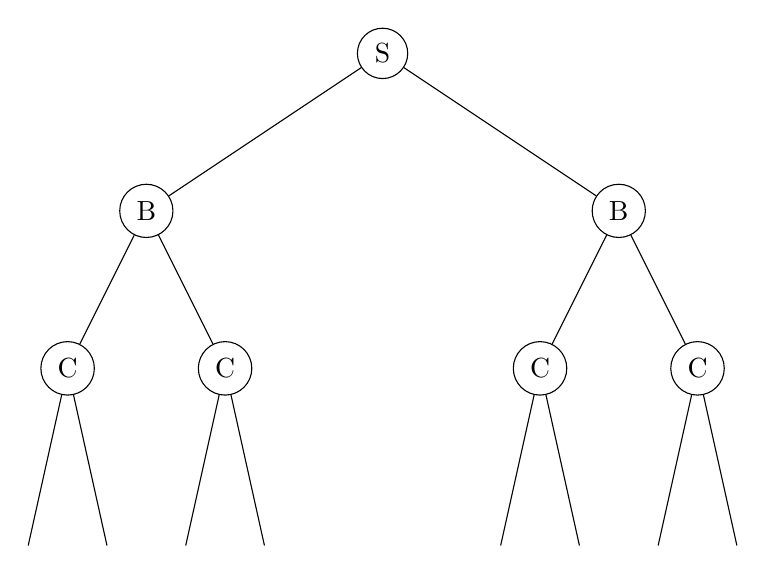
\begin{tikzpicture}
        \node [draw,circle](a)at(4,6){S};
        \node [draw,circle](b1)at(1,4){B};
        \node [draw,circle](b2)at(7,4){B};
        \node [draw,circle](c1)at(0,2){C};
        \node [draw,circle](c2)at(2,2){C};
        \node [draw,circle](c3)at(6,2){C};
        \node [draw,circle](c4)at(8,2){C};

        \draw (a) -- (b1);
        \draw (a) -- (b2);       
        \draw (b1) -- (c1);
        \draw (b1) -- (c2);
        \draw (b2) -- (c3);
        \draw (b2) -- (c4);
        \draw (c1) -- (-1/2,-1/4);
        \draw (c1) -- (1/2,-1/4);
        \draw (c2) -- (3/2,-1/4);
        \draw (c2) -- (5/2,-1/4);
        \draw (c3) -- (11/2,-1/4);
        \draw (c3) -- (13/2,-1/4);
        \draw (c4) -- (15/2,-1/4);
        \draw (c4) -- (17/2,-1/4);
    \end{tikzpicture}
    \caption{Repeated state without redundant path elimination}
    \label{fig:repeated_state_without_rpe}
\end{figure}

\noindent
Generally, 
\begin{outline}
    \1 UCS + Greedy search = $A^{*}$ without redundant path elimination
    \1 $A^{*}$ = UCS + Greedy search + redundant path elimination
\end{outline}

\noindent
The algorithm of redundant path elimination \emph{(First version: the closed set, not the path deletion version)} is shown as below: \\ \\
\textbf{Input:}
\tabto{5mm} a graph,
\tabto{5mm} a set of start nodes,
\tabto{5mm} Boolean procedure $goal(n)$ that tests if $n$ is a goal node. \\
\emph{frontier} := {$<s>$: $s$ is a start node} \\
\textcolor{red}{\emph{closed} := \{\}} \\
\textbf{while} \emph{frontier} is not empty:
\tabto{5mm} \textbf{select} and \textbf{remove} path $<n_{0},...,n_{k}>$ from \emph{frontier}
\tabto{5mm} \textcolor{red}{\textbf{if} $n_{k} \notin closed$ \textbf{then}}
\tabto{10mm} \textcolor{red}{add $n_{k}$ to \emph{closed}}
\tabto{10mm} \textbf{if} \emph{goal($n_{k}$)}
\tabto{15mm} \textbf{return} $n_{0},...,n_{k}$
\tabto{10mm} \textbf{for every} neighbor $n$ of $n_{k}$
\tabto{15mm} \textbf{add} $n_{0},...,n_{k}$ to \emph{frontier} \\
\textbf{end while} \\

\subsection{$A^{*}$ went wrong}
\noindent
Problem: When $A^{*}$ gone wrong?. If the heuristics is \textbf{\textcolor{red}{not consistent}}. There are two options: consistent heuristics or repair the frontier
\begin{enumerate}
    \item Consistent heuristics: ensure that the first "selected" path to a node always has lowest cost, thus, we can directly prune node by closed set without considering. \emph{(This can only work for consistent admissble heuristics)}
    \item Repair the frontier: if there is a path $p = <s,...,n,...,m>$ on the frontier and a path $p^{\prime}$ to $n$ such that $g(p^{\prime} \ge g(p))$ then remove $p^{\prime}$ from the frontier. \emph{(This can work for any admissible heuristics)}
\end{enumerate}

\subsubsection{Consistent heuristics}
\noindent
Difference between admissibility and consistency. But the main idea for both is "estimated heuristic cost $\le$ actual consts". Generally, \textbf{consistency $\rightarrow$ admissibility}. Consistency makes $A^{*}$ having a \textbf{f-contour}, and increase this \textbf{"f-contour"} one by one.
\begin{outline}
    \1 Admissibility: from A to G, heuristic cost $\le$ actual cost to goal (for whole)
        \2 $h(A) \le$ actual cost from A to G
    \1 Consistency: for each path from power set of from A to G, heuristic "arc" cost $\le$ actual cost for each arc
        \2 $h(A) - h(C) \le$ cost (A to C)
\end{outline}

\subsubsection{repair frontier}
For repairing the frontier, we need to compare new repeated path, and the state in the current path, the algorithm is shown as below: \textbf{(no closed set exist)} \\

\noindent
\tabto{0mm} \textbf{Input:}
\tabto{5mm} a graph,
\tabto{5mm} a set of start nodes,
\tabto{5mm} Boolean procedure $goal(n)$ that tests if $n$ is a goal node.
\tabto{0mm} \emph{frontier} := {$<s>$: $s$ is a start node}
\tabto{0mm} \textcolor{red}{\st{\emph{closed} := \{\}}}
\tabto{0mm} \textbf{while} \emph{frontier} is not empty:
\tabto{5mm} \textbf{select} and \textbf{remove} path $<n_{0},...,n_{k}>$ from \emph{frontier}
\tabto{5mm} \textcolor{red}{\st{\textbf{if} $n_{k} \notin closed$ \textbf{then}}}
\tabto{10mm} \textcolor{red}{\st{add $n_{k}$ to \emph{closed}}}
\tabto{5mm} \textcolor{blue}{\textbf{if} \emph{goal($n_{k}$)}}
\tabto{10mm} \textcolor{blue}{\textbf{return} $n_{0},...,n_{k}$}
\tabto{5mm} \textcolor{blue}{\textbf{for every} neighbor $n$ of $n_{k}$}
\tabto{10mm} \textcolor{blue}{\textbf{add} $n_{0},...,n_{k}$ to \emph{frontier}} 
\tabto{5mm} \textcolor{blue}{\textbf{if} there are $p = <s,t_{1},t_{2},...,t_{k},i,...,m>$ and $p^{\prime} = <s,s_{1},s_{2},...,s_{l},i>$ on the frontier and $g(p^{\prime}) \ge g(p)$} 
\tabto{10mm} \textcolor{blue}{\textbf{then} remove all such $p^{\prime}$} 
\tabto{0mm} \textbf{end while} \\

\subsection{Iterative Deepening $A^{*}$}
Idea from $A^{*}$ with consistent heuristics, with increasing "f-contour". Can we do this \textbf{iteratively}? Get DFS\'s space advantages with $A^{*}$ time. The difference between ID and ID$A^{*}$ is \textbf{how to choose "contour limit"}. The ID$A^{*}$ usually combined with loop breaking instead of redundant path elimination (this is not $A^{*}$), as this requires to store all generated nodes (closed set).
\begin{outline}
    \1 For ID, just do a DFS, if no solution, just limit = limit + 1
    \1 For ID$A^{*}$, if no solution, \textcolor{blue}{\textbf{use the smallest f value as the next contour.}}
\end{outline}

\noindent
The algorithm of ID$A^{*}$ is shown as below: \\ \\
\tabto{0mm} \textbf{procedure f-limited-search (}
\tabto{5mm} \textbf{input:} a graph,
\tabto{5mm} a set of start nodes,
\tabto{5mm} Boolean procedure \emph{goal(n)} that tests if \emph{n} is a goal node,
\tabto{5mm} \textcolor{red}{$f_{bound}$: positive number}
\tabto{0mm} )
\tabto{0mm} \emph{frontier} := {$<s>$: $s$ is a start node}
\tabto{0mm} $f_{next}$ := $\infty$
\tabto{0mm} \textbf{while} \emph{frontier} is not empty:
\tabto{5mm} \textbf{select} and \textbf{remove} first $p = <n_{0},...,n_{k}>$ from \emph{frontier}
\tabto{10mm} \textbf{if} $goal(n_{k})$ \textbf{then return} $p$
\tabto{10mm} \textbf{for every} neighbor $n$ of $n_{k}$
\tabto{15mm} compute $f_{n} = f(<n_{0},...,n_{k},n>)$
\tabto{15mm} \textbf{if} $f_{n} \le f_{bound}$
\tabto{20mm} \textbf{then add} $<n_{0},...,n_{k},n>$ to front of \emph{frontier}
\tabto{15mm} \textbf{if} $f_{n} > f_{found}$ and $f < f_{next}$
\tabto{20mm} \textbf{then} $f_{next} := f_{n}$
\tabto{0mm} \textbf{end while}
\tabto{0mm} \textbf{return} $f_{next}$

The properties of ID$A^{*}$ is shown as below:
\begin{outline}
    \1 Time complexity: worst case like $b^{0} + (b^{0} + b^{1}) + (b^{0} + b^{1} + b^{2}) + ... + (b^{0} + b^{1} + ... + b^{N}) = ...$, \textcolor{red}{which is $O(b^{\frac{C^{*}}{\epsilon}})$, as ID is $O(b^{d})$}
        \2 with b: branching factor, $C^{*}$: solution cost, arc cost (cost between 2 neighbor nodes) at least $\epsilon$ shallowest-solution depth, s: shallowest-solution depth
    \1 Space complexity: \textcolor{red}{$O(b \times \frac{C^{*}}{\epsilon})$ worst case $h=0$, as ID is $O(b \times s)$}
        \2 with b: branching factor, $C^{*}$: solution cost, arc cost (cost between 2 neighbor nodes) at least $\epsilon$, s: shallowest-solution depth
    \1 Completeness: yes due to optimal
    \1 Optimal: yes, under same situation as UCS + Greedy Search \emph{(Consistent admissible heuristics or redundant path elimination)}
\end{outline}


\subsection{Summary}
\begin{enumerate}
    \item The best heuristics $f(n) = g(n) + h(n)$ is an \textbf{admissble heuristics} with the combination of Uniformed Cost Search and Greedy Search.
    \item Coming up with a good admissible heuristics is important (larger -> better -> closer to the $h^{*}(n)$ (actual value), but also should be (for all nodes n) smaller than $h^{*}(n)$)
    \item \textbf{Heuristics design} is key for searching problem!
    \item Uniformed search vs. Informed Search = with or without \textbf{"heuristics"}
    \item $f(n) = g(n) + h(n)$, \textbf{difference choices $\rightarrow$ difference algorithms}, where without $g(n)$ is Greedy search, and without $h(n)$ is UCS, with both $g(n)$ and $h(n)$ is $A^{*}$ without redundant path elimination.
    \item Important \textbf{FOUR} properties for an algorithm: Time complexity, Space complexity, Completeness, Optimality.
\end{enumerate}

\pagebreak
\section{Constraint Sastification Problems}
\subsection{Overview}
Two different tasking: planning and identification
\begin{enumerate}
    \item Planning: sequences of actions: path is important
    \item Identification: assignments to variables: goal is important (CSP)
\end{enumerate}

\noindent
What is CSP?
\begin{outline}
    \1 A special subset of search problems
    \1 State is defined by varaible $X_{i}$ with values from a domain $D$
    \1 Goal is a set of \textbf{constraints} specifying allowable combination of values for subsets of variables
\end{outline}

\noindent
For example, the N-Queens problem: \\
\begin{outline}
    \1 Variables: $X_{i,j}$
    \1 Domains: $D = {0,1}$
    \1 Constraints: \textbf{(not allow touch together (1,1))}
        \2 $\forall i,j,k (X_{i,j},X_{i,k} \in {(0,0),(0,1),(1,0)})$
        \2 $\forall i,j,k (X_{i,j},X_{k,j} \in {(0,0),(0,1),(1,0)})$
        \2 $\forall i,j,k (X_{i,j},X_{i+k,j+k} \in {(0,0),(0,1),(1,0)})$
        \2 $\forall i,j,k (X_{i,j},X_{i+k,j-k} \in {(0,0),(0,1),(1,0)})$
        \2 $\sum_{i,j} X_{i,j} = N$
\end{outline}

\subsection{Variaties of CSP}
Variables can be classified as: \textbf{discrete variables} and \textbf{continuous variables}. And the discrete variable can be further classified as \textbf{finite domain} and \textbf{infinite domains}. \\
Constrains can be classified as \textbf{hard constraints} and \textbf{soft constraints}. Hard constraint includes \textbf{unary constraint} involing a single variable: $SA \neq green$, or \textbf{binary constraint} involing pairs of variable: $SA \neq WA$, or even \textbf{higher-order constraints} involing 3 or more variables: $O + O = R + 10 \times X_{1}$. \textbf{Preferences} (soft constraint) is also important, which will be used in Constrained Optimization Problem.

\subsection{Solution to CSP}
The standard search formulation is defined as below (initial $\rightarrow$ assigning values to unassigned varaibles $\rightarrow$ check goal test):
\begin{enumerate}
    \item Initial state: the empty assignment, \{\}
    \item Successor funtion: assign a value to an unassigned variables
    \item Goal test: the current assignment is complete and satisfies all constraints
\end{enumerate}

\subsection{Backtracking}
Backtracking search is the basic uniformed algorithm for solving CSPs. DSP with two improvements below is called "backtracking search". In CSP, DFS is better than BFS since BFS will check layer by layer which is unnecessary. 
\begin{enumerate}
    \item One variable at time - only consider assignments to a single variable at each step
    \item Check constraints as you go - consider only values which do not conflict previous assignments
\end{enumerate}

\noindent
The algorithm of backtracking search is shown as below: \\
\tabto{0mm} \textbf{function} BACKTRACKING-SEARCH(csp) \textbf{returns} solution/ failure
\tabto{5mm} \textbf{return} RECURSIVE-BACKTRACKING(\{\},csp)
\\
\tabto{0mm} \textbf{function} RECURSIVE-BACKTRACKING(assignment, csp) \textbf{return} solution/ failure
\tabto{5mm} \textbf{if} assignment is complete \textbf{then return} assignment
\tabto{5mm} var $\leftarrow$ SELECT-UNASSIGNED-VARIABLE(VARIABLE[csp], assignment, csp)
\tabto{5mm} \textbf{for each} value \textbf{in} ORDER-DOMAIN-VALUES(var, assignment, csp) \textbf{do}
\tabto{10mm} \textbf{if} value is consistent with assignment given CONSTRAINTS[csp] \textbf{then}
\tabto{15mm} add \{var = value\} to assignment
\tabto{15mm} var $\leftarrow$ RECURSIVE-BACKTRACKING(assignment, csp)
\tabto{15mm} \textbf{if result $\neq$ failure}
\tabto{20mm} \textbf{then return} result \textcolor{cyan}{\emph{\% Find answer, so return result}}
\tabto{20mm} \textbf{else} remove \{var = value\} from assignment
\tabto{5mm} \textbf{return} failure  \textcolor{cyan}{\emph{\% No completed solution found, so return failure}}


\noindent
\\ As we can see above, Backtracking = DFS + variable-ordering \emph{(select one variable)} + fail-on-violation \emph{(check constraint)}

\subsection{Improvement on Backtracking}
The improvement can be applied on three aspects: Ordering, Filtering and Structure:
\begin{enumerate}
    \item Ordering - which should be next, similar to heuristics
    \item Filtering - can we detect inevitable failure in advance?
    \item Structure - can we exploit the problem structure?
\end{enumerate}

\subsubsection{Filtering}
\noindent
Filtering: keep track of domains for unassigned variables and cross off bad options \\
\textbf{Forward checking (FC)}: Corss off values that violate a constraint when added to the existing assignment; but not provide early detection for all failures. \textbf{Assign values to unassigned variables to check, and backtrack.} \textbf{Constraint propagation}: reason from constraint to constraint. \\
\textbf{Consistency of a single arc (AC-3)}: An arc X $\rightarrow$ Y is consistent iff for \emph{every} x in the tail there is \emph{some} y in the head which could be assigned without violating the constraint. Important: if X loses a value, neighbors of X need to be rechecked! Arc consistency detects failure earlier than forward checking. It checks \textbf{all} arcs are consistency once time. \\
Both constraint propagation and consistency of a single arc can be run as a \textbf{preprocessor} or \textbf{after each assignment}. \\
The algorithm is shown as below: \\ \\
\tabto{0mm} \textbf{function} AC-3(csp) \textbf{returns} false if an inconsistency is found and true otherwises
\tabto{5mm} queue $\leftarrow$ a queue of arcs, initially all the arcs in csp \textcolor{cyan}{\emph{\% arcs: double direction ($X_{i},X_{j}$) and ($X_{j},X_{i}$) are different}}
\tabto{5mm} \textbf{while} queue is not empty \textbf{do}
\tabto{10mm} ($X_{i},X_{j}$) $\leftarrow$ POP(queue)
\tabto{10mm} \textbf{if} REVISE(csp, $X_{i}$, $X_{j}$) \textbf{then}
\tabto{15mm} \textbf{if} size of $D_{i}$ = 0 \textbf{then return} false
\tabto{15mm} \textbf{for each $X_{k}$ in $X_{i}$.NEIGHBORS - \{$X_{j}$\} do}
\tabto{20mm} add ($X_{k}$, $X_{i}$) to queue
\tabto{5mm} \textbf{return} true

\tabto{0mm} \textbf{function} REVISE(csp, $X_{i}$, $X_{j}$) \textbf{returns} true iff we revise the domain of $X_{i}$
\tabto{5mm} revised $\leftarrow$ false
\tabto{5mm} \textbf{for each $x$ in $D_{i}$ do}
\tabto{10mm} \textbf{if} no value $y$ in $D_{j}$ allows ($x$,$y$) to satisfy the constraint between $X_{i}$ and $X_{j}$ \textbf{then} \\
\tabto{15mm} delete $x$ from $D_{i}$
\tabto{15mm} revised $\leftarrow$ true
\tabto{5mm} \textbf{return} revised \\

\noindent
Difference between forward checking and arc consistency: forward check is global and arc consistency is local (may not detect failure as more as forward check (the global)). More further comparison is shown as below: 
\begin{outline}
    \1 Filtering with Forward Checking (FC)
        \2 after assinging one variable, check the constraints that involve this variables
    \1 Filtering with Arc Consistency (AC3)
        \2 like FC, but if a variable changed, also check all constraints involing this variable (except itself)
\end{outline}

\subsubsection{Ordering}
There are two types of ordering, as shown below. But there is a common principle: \textbf{fail-first}.
\begin{enumerate}
    \item Variable ordering - which one to assign first?
    \begin{enumerate}
        \item Minimum Remaining Values
        \item Most Constratining Variables
    \end{enumerate}
    \item Value ordering - which value to try first?
    \begin{enumerate}
        \item Least Constraining Value
    \end{enumerate}
\end{enumerate}

\noindent
Minimum Remaining Values: choose the variable with the fewest legal left values in its domain $\rightarrow$ less values means less steps to iterate its remaining values $\rightarrow$ easy to check whether fail or success, fail-first. It is also called "Most Constrained Variable" \\

\noindent
Most Constraining Variables: choose the variable with the most constraints (only counting constraints involving other unassigned variables) $\rightarrow$ most constraints $\rightarrow$ easier to fail $\rightarrow$ fail-first. It is also called "max degree heuristics" \\

\noindent
Least Constraining Value: \textcolor{red}{given a choice of variable, choose the least constraining value.}Least value $\rightarrow$ closer to threshold $\rightarrow$ easier to delete. \textcolor{red}{$\leftarrow$ My guessing}. Why least rather than most? You can do this with most, actually.

\subsubsection{Structure}
\textbf{Independent substructure:} Some structure can be broken into subproblems, which can significantly improve the efficiency. Similar to Bi-direction search, from $O(b^{m})$ to $O(2 \times b^{\frac{m}{2}})$. \\
\textbf{Value symmetry:} in many CSP problems, there are many symmetries, we can reduce the search space by using \textbf{symmetry breaking constraints.}

\subsection{Constraint Optimization}
COP = Constraint Optimization Problem. It uses "branch-and-bound", similar to uniformed search. \\
\textbf{Key idea:} 
\begin{enumerate}
    \item maintain the 'best' objective value so far
    \item constrain solutions to be better than the 'best'
\end{enumerate}

\subsection{Summary}
\begin{enumerate}
    \item CSPs are a special kind of search problem
    \begin{enumerate}
        \item States are partial assignments
        \item Goal test defined by constraints
    \end{enumerate}
    \item Basic solution: backtracking search
    \item Speed-up
    \begin{enumerate}
        \item Filtering - FC, AC3
        \item Ordering - Minimum Remaining Values, Most Constraining Variables, Least Constraining Value
        \item Structure - substructure, symmetry breaking constraints
        \item Optimization - branch-and-bound
    \end{enumerate}
\end{enumerate}

\pagebreak
\section{Pattern mining}
\subsection{Overview}
Is to find interesting and actionable patterns and models in the data. \\

\noindent
Example: Recommender System \\
Terminology of datasets:
\begin{outline}
    \1 Itemsets
        \2 the special case where all attributes are boolean
        \2 a set of possible items $\mathscr{I}$
        \2 each example $e \subseteq \mathscr{I}$
        \2 each hypothesis $h \subseteq \mathscr{I}$
        \2 hypothesis $h$ covers example $e$ iff $h \subseteq e$ 
        \2 $h_{1}$ is more general than $h_{2}$ iff $h_{1} \subseteq h_{2}$, $h_{1}$ has less specific items, which means it is less specific
        \2 \textbf{hypothesis = pattern}
\end{outline}

\subsection{Frequent itemset mining}
\tabto{0mm} \textbf{Given:}
\tabto{5mm} a set of possible item $\mathscr{I} = {i_{1},...,i_{n}}$,
\tabto{5mm} a dataset $D$
\tabto{5mm} a threshold $c$
\tabto{0mm} \textbf{Find} all itemsets $I \subseteq \mathscr{I}$ such that $I$ is frequent in $D$, i.e., $freq(I,D) \ge c$. \\ 

\noindent
\textbf{"covers":} 
\begin{outline}
    \1 $h_{1}$ covers $h_{2}$ means $h_{1}$ is more general than $h_{2}$, i.e., \{s,b,c\} covers \{s,b,c\}, \{s,b,c,m\}
    \1 more examples, \{s,b\} covers \{s,b\}, \{s,b,c\}, \{s,b,c,m\}
\end{outline}

\subsection{Search space}
Adding more definition on \emph{Itemsets}
\begin{outline}
    \1 most general element: \{\}
    \1 most specific element: $\mathscr{I}$
\end{outline}

\noindent
As we see from Figure~\ref{fig:generality_ordering_lattice} and Table~\ref{tab:generality_ordering_lattice}, if the minimal freq threshold $c = 1$, $D = \{<s,b>\}$
\begin{outline}
    \1 $freq(\{\},D) = 1$
    \1 $freq(\{s\},D) = 1$
    \1 $freq(\{b\},D) = 0$
    \1 $freq(\{s,b\},D) = 0$
\end{outline}

\noindent
For minimal freq threshold $c = 1$, the answer would be \textbf{\{\}} and \textbf{\{s\}}.

\begin{table}[htbp]\footnotesize
    \centering
    \caption{Table for generality ordering lattice for \{s,b\}}
    \begin{tabularx}{4cm}{X|X}
    \toprule
    \textbf{s}&\textbf{b} \\
    \hline
    True&False \\
    \bottomrule
    \end{tabularx}
    \label{tab:generality_ordering_lattice}
\end{table}

\begin{figure}[htbp]
    \centering
    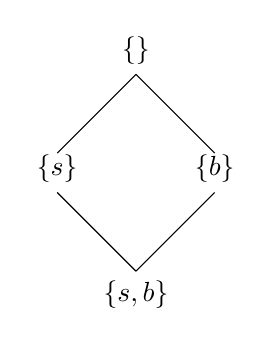
\begin{tikzpicture}
        \draw (0,5/2) -- (-1,3/2); 
        \draw (0,5/2) -- (1,3/2);
        \draw (-1,1) -- (0,0);
        \draw (1,1) -- (0,0);    

        \draw (0,5/2) node[above]{$\{\}$};
        \draw (-1,1) node[above]{$\{s\}$};
        \draw (1,1) node[above]{$\{b\}$};
        \draw (0,0) node[below]{$\{s,b\}$};
    \end{tikzpicture}
    \caption{Figure for generality ordering lattice for \{s,b\}}
    \label{fig:generality_ordering_lattice}
\end{figure}

\noindent
"Anti-monotonicity" principle: if $I_{1} \subseteq I_{2}$ (that is, $I_{1}$ is more general than $I_{2}$ then $freq(I_{1},D) \ge freq(I_{2},D)$, since it has more supersets) \\

\noindent
There are two borders: specific borders and general borders. 
\begin{enumerate}
    \item S-set = \{$I \subseteq \mathscr{I} | I$ satisfies min and max frequency thresholds, and there is no $J \subseteq \mathscr{I}$ that is strictly more specific than $I$ and also satisfies the thresholds\}. $\rightarrow$ meaning that \textbf{S is the most specific solution}, it contains all maximall solutions, solution that cannot be extended with extra items. 
    \item G-set = \{$I \subseteq \mathscr{I} | I$ satisfies min and max frequency thresholds, and there is no $J \subseteq \mathscr{I}$ that is strictly more geeneral than $I$\}. $\rightarrow$ meaning that \textbf{G is the most general solution}, it contains all minimal solutions, solution that cannot be deleted.
\end{enumerate}

\noindent
Concept-learning = 100\% frequency on the positives and 0\% frequency on the negatives.

\subsection{Enumeration Algorithms}
The naive algorithm for frequent itemset mining is shown as below: \\
\tabto{0mm} \textbf{Input:}
\tabto{5mm} a set of transactions $D$,
\tabto{5mm} a set of items $\mathscr{I}$,
\tabto{5mm} a frequency threshold $c$.
\tabto{0mm} Queue = \{\{\}\} \textcolor{cyan}{\emph{\% Empty set is also a itemset}}
\tabto{0mm} \textbf{for all} $I \in Queue$ \textbf{do}
\tabto{5mm} \textbf{if} $freq(I,D) \ge c$
\tabto{10mm} \textbf{then} output I
\tabto{10mm} add all $I \cup \{i\}$ to Queue (with $i \in \mathscr{I} - I$) \textcolor{cyan}{\emph{\% Add, s,c,b,m to \{\} to make \{s\}, \{c\}, \{b\}, \{m\}}}
\tabto{0mm} \textbf{end for}

\noindent
\\ Improvement: the naive algorithm has too many redundant examples, "lexicographic order" can be used to improve the efficiency. Symmetry breaking: impose the order $s > m > c > b$, and never add an element to a set $I$ if it smaller than the smallest element in the set. \emph{Every set is only generated once and we get a tree instead of a graph.} The algorithm is shown as below \textbf{(min + max + lexicographic)}:

\tabto{0mm} \textbf{Input:}
\tabto{5mm} a set of pos transactions \emph{Pos},
\tabto{5mm} a set of neg transactions \emph{Neg},
\tabto{5mm} a set of items $\mathscr{I}$,
\tabto{5mm} frequency thresholds $t_{1}, t_{2}$
\tabto{0mm} Queue = \{\{\}\}
\tabto{0mm} \textbf{for all} $I \in Queue$ \textbf{do}
\tabto{5mm} \textbf{if} $freq(I, Pos) > t_{1}$
\tabto{10mm} \textbf{then if} \textcolor{red}{$freq(I, Neg) \le t_{2}$} \textcolor{cyan}{\emph{\% This Neg can be Pos, too, but the truth meaning is $t^{\prime} \ge freq(I, Pos) \le t^{\prime \prime}$}}
\tabto{15mm} \textbf{then} output $I$
\tabto{20mm} add all $I \cup \{i\}$ to Queue (with $i \in \mathscr{I} - I$ and \textcolor{red}{$i$ lexicographically smaller than elements of $I$})
\tabto{0mm} \textbf{end for}

\subsection{Summary}
\begin{enumerate}
    \item The basic concept-learning - frequent itemsets mining
    \item min + max is just  ont type of constraints
    \item 100\% frequency on positives and 0\% on negatives = concept-learning with version spaces
    \item Frequent patterns can be turned in association rules to make predictions - similar to Naive Bayes (Probabilistic Machine Learning)
\end{enumerate}

\pagebreak

\section{Game tree}
\subsection{Games}
There are different kind of games: 
\begin{outline}
    \1 Deterministic or stochastic game
    \1 Multi-player or single player game
    \1 Zero-sum or general game
    \1 Board game \textcolor{blue}{$\leftarrow$ we will focus on this!}
\end{outline}

\noindent
A good game program/ strategy should have the properties that
\begin{enumerate}
    \item delete \textbf{irrelevant branches} of the search tree
    \item use \textbf{goof evaluation functions} for in-between states
    \item \textbf{look ahead} as many moves as possible
\end{enumerate}

\subsection{Minimax}
\subsubsection{Terminology}
Soem terminology of two-person board games:
\begin{outline}
    \1 Players are \textbf{min} and \textbf{max}, where max begins
    \1 \textbf{Initial} position
    \1 \textbf{Operators}, actions
    \1 \textbf{Game tree} is the search tree generated from the possible moves
    \1 \textbf{Termination} test, determines when the game is over and what the \textbf{value of final state} is
    \1 \textbf{Strategy}
\end{outline}

\subsubsection{Algorithm}
\noindent
For minimax algorithm, we use DFS to generate the game tree. We will apply \textbf{utility function}/ heuristics function to each terminal state. During the minimax, max should have the highest value, and min will always choose the worst-value step for max (they are opponents!). The algorithm is shown as below: 

\tabto{0mm} \textbf{function} MINIMAX-SEARCH(game, state) \textbf{returns} an action
\tabto{5mm} player $\leftarrow$ game.TO-MOVE(state)
\tabto{5mm} value,move $\leftarrow$ MAX-VALUE(game,state)
\tabto{5mm} \textbf{return} move

\tabto{0mm} \textbf{function} MAX-VALUE(game,state) \textbf{returns} a (utility,move) pair
\tabto{5mm} \textbf{if} game.IS-TERMINAL(state) \textbf{then return} game.UTILITY(state,player),null
\tabto{5mm} v $\leftarrow$ $- \infty$
\tabto{5mm} \textbf{for each $a$ in} game.ACTIONS(state) \textbf{do}
\tabto{10mm} v2,a2 $\leftarrow$ MIN-VALUE(game,game.RESULT(state,a))
\tabto{10mm} \textbf{if} v2 $>$ v \textbf{then}
\tabto{15mm} v,move $\leftarrow$ v2,a
\tabto{5mm} \textbf{return} v,move

\tabto{0mm} \textbf{function} MIN-VALUE(game,state) \textbf{returns} a (utility,move) pair
\tabto{5mm} \textbf{if} game.IS-TERMINAL(state) \textbf{then return} game.UTILITY(state,player),null
\tabto{5mm} v $\leftarrow$ $+ \infty$
\tabto{5mm} \textbf{for each $a$ in} game.ACTION(state) \textbf{do}
\tabto{10mm} v2,a2 $\leftarrow$ MAX-VALUE(game,game.RESULT(state,a))
\tabto{10mm} \textbf{if} v2 $<$ v \textbf{then}
\tabto{15mm} v,move $\leftarrow$ v2,a
\tabto{5mm} \textbf{return} v,move

\subsubsection{Evaluation function}
The evaluation function is important! Some examples are shown below:
\begin{outline}
    \1 Material value: pawn/1, knight/3, queen/9
    \1 Other: king safety, good pawn structure
    \1 Rule of thumb: three-point advantage
\end{outline}

\noindent
The preffered evaluation functions are \textbf{weighted, linear functions}: $w_{1}f_{1} + w_{2}f_{2} + ... + w_{n}f{n}$, where $w_{i}$ are the weights and the $f_{i}$ are the features of the board. However, it has a strong assumption that all of features are \textbf{independent}, which is unrealistic.

\subsubsection{Stopping criteria}
Stopping critiera can be fixed-depth or iterative deepening (when time is over.) However, only stop and evaluate in \textbf{quiescent positions} that will not cause large fluctuations. Because we do not know what happen if so large fluctuations happen may cause $\rightarrow$ \textcolor{blue}{\textbf{horizon effect:} try to delay lose but fail and with more cost}.

\subsection{Alpha-Beta Search}
It is an optimization of minimax algorithm, which helps improve its efficiency. Instead of generating tree $\rightarrow$ propogating the values upwards in the tree. We try to \textbf{interleave these two steps}, meaning that exploit $\rightarrow$ propogate $\rightarrow$ prune $\rightarrow$ exploit $\rightarrow$ propogate $\rightarrow$ prune. Some terminology is shown as below:
\begin{outline}
    \1 The temporary values at MAX-nodes are alpha($\alpha$) values
    \1 The temporary values at MIN-nodes are beta($\beta$) values
\end{outline}

\noindent
Minimax algorithm with DFS, it provides the \textbf{same result} as the complex minimax search to the same depth because only irrelevant nodes are eliminated.
\begin{outline}
    \1 ALPHA = the value of the best choice we have found so far at any choice point along the path for MAX
        \2 ALPHA value can \textbf{never devrease}
    \1 BETA = the value of the best choice we have found so far at any choice point along the par for MIN
        \2 BETA value can \textbf{never increase}
\end{outline}

\noindent
The Alpha-Beta (pruning) principle is shown as below:
\begin{outline}
    \1 If an \textbf{ALPHA-value is larger or equal than the BETA-value} of a descendant node: stop generation of the children of the descentdant
    \1 If a \textbf{BETA-value is smaller or equal than the ALPHA-value} of a descendant node: stop generation of the children of the descendant
\end{outline}

\noindent
The algorithm for ALPHA-BETA is shown as below:

\tabto{0mm} \textbf{function} MINIMAX-SEARCH(game,state) \textbf{returns} an action
\tabto{5mm} player $\leftarrow$ game.TO-MOVE(state)
\tabto{5mm} value,move $\leftarrow$ MAX-VALUE(game,state,$- \infty$,$+ \infty$)
\tabto{5mm} \textbf{return} move

\tabto{0mm} \textbf{function} MAX-VALUE(game,state,$\alpha$,$\beta$) \textbf{returns} a (utility,move) pair
\tabto{5mm} \textbf{if} game.IS-TERMINAL(state) \textbf{then return} game.UTILITY(state,player),null
\tabto{5mm} v $\leftarrow$ $- \infty$
\tabto{5mm} \textbf{for each $a$ in} game.ACTIONS(state) \textbf{do}
\tabto{10mm} v2,a2 $\leftarrow$ MIN-VALUE(game,game.RESULT(state,a),$\alpha$,$\beta$)
\tabto{10mm} \textbf{if} v2 $>$ v \textbf{then}
\tabto{15mm} v,move $\leftarrow$ v2,a
\tabto{15mm} $\alpha \leftarrow$ MAX($\alpha$,v) \textcolor{cyan}{\emph{\% prepare $\alpha$ for MIN}}
\tabto{10mm} \textbf{if} v $> \beta$ \textbf{then reutrn} v,move \textbf{then return} result \textcolor{cyan}{\emph{\% ALPHA-BETA pruning, just return}}
\tabto{5mm} \textbf{return} v,move

\tabto{0mm} \textbf{function} MIN-VALUE(game,state,$\alpha$,$\beta$) \textbf{returns} a (utility,move) pair
\tabto{5mm} \textbf{if} game.IS-TERMINAL(state) \textbf{then return} game.UTILITY(state,player),null
\tabto{5mm} v $\leftarrow$ $+ \infty$
\tabto{5mm} \textbf{for each $a$ in} game.ACTION(state) \textbf{do}
\tabto{10mm} v2,a2 $\leftarrow$ MAX-VALUE(game,game.RESULT(state,a),$\alpha$,$\beta$)
\tabto{10mm} \textbf{if} v2 $<$ v \textbf{then}
\tabto{15mm} v,move $\leftarrow$ v2,a
\tabto{15mm} $\beta \leftarrow$ MIN($\beta$,v) \textcolor{cyan}{\emph{\% prepare $\beta$ for MAX}}
\tabto{10mm} \textbf{if} v $\le \alpha$ \textbf{then return} v,move \textcolor{cyan}{\emph{\% ALPHA-BETA pruning, just return}}
\tabto{5mm} \textbf{return} v,move

\noindent
\\ The Gain: best case. If at every layer: the best node is the left-most one \textbf{(perfectly ordered tree)}. In the best case, the search expenditure is reduced to $O(b^{\frac{d}{2}})$

\subsection{Expectiminimax}
If there is posibility, stochastic instead of deterministic.
\tabto{0mm} $d_{i}$: possible dice roll
\tabto{0mm} $P(d_{i})$: probability of obtaining that roll
\tabto{0mm} $EXPECTIMINIMAX(s) = $
\tabto{5mm} $UTILITY(s)$ if $IsTerminal(s)$
\tabto{5mm} $max_{a} EXPECTIMINIMAX(Result(s,a))$ if $ToMove(s) = MAX$
\tabto{5mm} $min_{a} EXPECTIMINIMAX(Result(s,a))$ if $ToMove(s) = MIN$
\tabto{5mm} $\sum_{d} P(d) \times EXPECTIMINIMAX(Result(s,d))$ if $ToMove(s) = CHANCE$
\tabto{0mm} $Result(s,d)$: attainable positions from $C$ with $d$

\subsection{Summary}
\begin{enumerate}
    \item A \textbf{game} can be defined by the initial state, the operator/actions, a terminal test, a utility function/ outcome of the game
    \item In two-player board game, \textbf{minimax algorithm} can be used.
    \item The \textbf{alpha-beta algorithm} produces the \textbf{same result} but it is more efficient because it just prunes away irrelevant branches.
    \item \textbf{Utility/heuristics} of some states will be determined by an \textbf{evaluation function}.
    \item Games of chance can be handled by some extension, EXPECTIMINIMAX.
    \item The success for different games is based on quite different methodologies.
\end{enumerate}

\pagebreak
\section{Planning}
\subsection{Overview}
Some lectures overview:
\begin{outline}
    \1 Algorithm fundamentals of search
        \2 Intro AI and Rational agents
        \2 Uniformed Search
        \2 Informed Search
    \1 Applications of search in deterministic environments
        \2 CSP
        \2 Pattern Mining
        \2 Game Tree
        \2 Planning
    \1 Application of search in stochastic environments
        \2 Markov Decision Processes
    \1 BDA
        \2 Intro to logic
        \2 SAT solving
        \2 Local Search
\end{outline}

\noindent
The planning we learn is \textbf{Goal Oriented Action Planning: STRIPS Planning.} Search for a plan that achieves that goal in the current state.

\subsection{STRIPS planning}
\subsubsection{Overview}
Typical description of a planning problem:
\begin{outline}
    \1 Initial state
    \1 Goal
    \1 Available actions
\end{outline}

\noindent
Typical solution of a planning problem: a sequence of actions when excuted in the initial state results in a state that satisfies the goal condition. (\textbf{A sequence of actions} that achieves the goal for \textbf{every application domain})

\noindent
Planning: the automatic discovery of such solutions. (\textbf{Find} such sequence of actions that achieves the goal for every application domain)

\subsubsection{Example: Blocks world domain}
\begin{outline}
    \1 Initial state: $s_{0}$
    \1 Goal: $g$
    \1 Available actions:
        \2 $move(A,table,B)$: move A from table to top of B
        \2 $move(A,B,table)$: move A from top of B to table
        \2 $move(A,C,B)$: move A from top of C to top of B (not from table)
\end{outline}

\begin{figure}[htbp]
    \centering
    \begin{subfigure}[t]{0.25\textwidth}
        \centering
        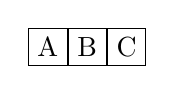
\begin{tikzpicture}
            \node [draw,rectangle](a)at(-1/2,0){A};
            \node [draw,rectangle](b)at(0,0){B};
            \node [draw,rectangle](c)at(1/2,0){C};     
        \end{tikzpicture}
        \caption{Initial state $s_{0}$}
        \label{fig:initial_state_in_BWD}
    \end{subfigure}
    \begin{subfigure}[t]{0.25\textwidth}
        \centering
        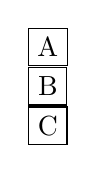
\begin{tikzpicture}
            \node [draw,rectangle](a)at(0,1){A};
            \node [draw,rectangle](b)at(0,1/2){B};
            \node [draw,rectangle](c)at(0,0){C};     
        \end{tikzpicture}
        \caption{Goal state $g$}
        \label{fig:goal_state_in_BWD}
    \end{subfigure}
    \caption{Initial state and Goal state for Blocks world domain}
    \label{fig:states_in_BWD}
\end{figure}

\noindent
In the beginning, we need to find a representation for the state and actions. For the state in blocks world is shown as below. For each state, the state should be \textbf{completely} specified based on the \textcolor{blue}{\textbf{Closed-World Assumption: any literal not mentioned in the description of the state are assumed to be false!}}.
\begin{outline}
    \1 On(b,x):
        \2 block b is on top of x, where x is another block 
    \1 Clear(x):
        \2 a block can be placed on the top of x
\end{outline}

\noindent
Thus, the initial state in Figure~\ref{fig:initial_state_in_BWD} are: $on(a,table)$, $on(b,table)$, $on(c,table)$, $clear(a)$, $clear(b)$, $clear(c)$. \textcolor{blue}{(Closed-World Assumption)} Additionally, the goal state in Figure~\ref{fig:goal_state_in_BWD} are: $clear(a)$, $on(a,b)$, $on(b,c)$, $on(c,table)$. \textcolor{blue}{(No Closed-World Assumption)}, we only need to satify the goal. (A state $s$ satisfies goal $g$ if it contains all literals in $g$, containing is okay, not exactly identified.)

\noindent
Next is the availble actions. It consists of \textbf{preconditions} and \textbf{effects}.
\begin{outline}
    \1 Preconditions: literals denoting what needs to be in the state for the action to be availble
    \1 Effects: literals denoting how the state is changing when action is applied
\end{outline}

\noindent
One of the avialble action is $move(b,x,y)$, meaning that move b from top of x to top of y. Anonther action can be $moveToTable(b,x)$ and $moveFromTable(b,x)$
\tabto{0mm} $move(b,x,y)$
\tabto{5mm} Preconditions:
\tabto{10mm} $on(b,x)$, $clear(b)$, $clear(y)$
\tabto{5mm} Effects:
\tabto{10mm} $\neg on(b,x)$, $\neg clear(y)$, $on(b,y)$, $clear(x)$ 
\tabto{0mm} $moveToTable(b,x)$
\tabto{5mm} Preconditions:
\tabto{10mm} $clear(b)$, $on(b,x)$
\tabto{5mm} Effects:
\tabto{10mm} $\neg on(b,x)$, $on(b,table)$, $clear(x)$
\tabto{0mm} $moveFromTable(b,x)$
\tabto{5mm} Preconditions:
\tabto{10mm} $clear(b)$, $clear(x)$
\tabto{5mm} Effects:
\tabto{10mm} $\neg on(b,table)$, $\neg clear(x)$, $on(b,x)$

\noindent
Why do we like formalism? Because it is easy for representation. STRIPS planning: finding a solution to the planning problem following a \textbf{state-based search:}
\begin{outline}
    \1 Init(\textcolor{orange}{where to start from})
    \1 Goal(\textcolor{orange}{when to stop searching})
    \1 Action(\textcolor{blue}{how to generate the "graph"})
\end{outline}

\noindent
When planning, there are two planning: 
\begin{outline}
    \1 Progression planning: forward state-based search \textcolor{red}{$\leftarrow$ mainly focus on}
    \1 Regression planning: backward state-based search
\end{outline}

\noindent 
The \textbf{\textcolor{blue}{pseudocode}} for progressing planning: - similar to backtracking
\begin{enumerate}
    \item Start from the initial state
    \item Check if the current state satisfies the goal
    \item Compute availble actions to the current state
    \item Compute the successor states
    \item Pick one of the \textbf{(not-visited)} successor states as the current state
    \item Repeat until a solution is found or the state space is exhausted \textcolor{red}{$\leftarrow$ similar to backtracking}
\end{enumerate}

\noindent
Is it guaranteed that progressive planning will find a solution if one exists? \textcolor{red}{$\leftarrow$ yes, if the state-space is finite} 

\noindent
But it will be very very slow, if we search the whole space-state (the worst case). \textcolor{red}{$\leftarrow$ heuristics needed!} We need heuristics that help progression planning pick the most promising states to investigate first

\subsection{Heuristics for STRIPS planning}
Analogy: $A^{*}$ search, evalution function = $f(s) = g(s) + h(s)$, where $g(s)$ from UCS and $h(s)$ from greedy search. Similar to the $A^{*}$ search, here we use $f(s)$ for STRIPS planning to pick the most promising one. Some of possible $h(s)$ and $g(s)$ can be as below. \emph{(Similarly, we need to check whether it is admissble heuristics to obtain the optimal solution)}
\begin{outline}
    \1 $g(s)$: number of literals that exists in the goal
    \1 $h(s)$: number of literals in the goal that are missing from s
\end{outline}

\noindent
The \textcolor{blue}{\textbf{pseudocode}} for \textcolor{blue}{\textbf{progressing planning}} applied with heuristics can be updated as below:
\begin{enumerate}
    \item Start from the initial state
    \item Check if the current state satisfies the goal
    \item Compute availble actions to the current state
    \item Compute the successor states
    \item Pick \textcolor{red}{\textbf{(the most promising}} successor states as the current state
    \item Repeat until a solution is found or the state space is exhausted \textcolor{red}{$\leftarrow$ similar to backtracking}
\end{enumerate}

\noindent
Alternatives: \textcolor{blue}{\textbf{pseudocode}} for \textcolor{blue}{\textbf{Regression planning }} is similar but invert the progressing planning:
\begin{enumerate}
    \item Start from the \textbf{goal} state as current state
    \item Check if the \textbf{initial state} satisfies the current state
    \item Compute the \textbf{relevant} and \textbf{consistent} actions for current state
    \item Compute the \textbf{predecessor} states (which is actually next state in this case)
    \item Pick \textcolor{red}{\textbf{(the most promising}} successor states as the current state
    \item Repeat until a solution is found from \textbf{goal state} to \textbf{initial state} or the state space is exhausted (no solution)
\end{enumerate}

\subsection{Summary}
\begin{enumerate}
    \item A generic formalism (easy to represent difficult space search, similar to ILP) for \textbf{representing} planning problem (a specific aspect in searching problem)
    \item Generic \textbf{search} procedures for finding a plan
    \begin{enumerate}
        \item Progressing planning (forward)
        \item Regression planning (backward, not discussed, only pseudocode)
    \end{enumerate}
    \item Application in many aspects, e.g., space, flight, robotics, etc.
\end{enumerate}


\pagebreak
\section{Markov Decision Process}
\subsection{Overview}
This section is about non-deterministic search, which is called stochastic search. First we can take Grid World as an example, which is shown below:

\begin{outline}
    \1 A maze-like problem
        \2 Agent move in the grid
        \2 Walls block the agent's path
    \1 Noisy movement - stochastic movement
        \2 $80\% \rightarrow$ correct direction, $20\% \rightarrow$ other (incorrect) directions.
    \1 The agent recives rewards each time step
        \2 Small living rewards (can be negative)
        \2 Big rewards at the end (negative or positive)
    \1 Goal: maximize sum of rewards
\end{outline}

\noindent
An MDP is defined as below. The MDP, the "markov" means actions outcomes depend only the current state, and the current, future and past are independent. It is similar to search, where the successor function could only depend on the current state (not the history). 
\begin{outline}
    \1 a set of states $s \in S$
    \1 a set of actions $ a \in A$
    \1 a transition function $T(s,a,s^{\prime})$
    \1 a reward function $R(s,a,s^{\prime})$
    \1 an initial state
    \1 some goal states (probably not)
\end{outline}

\noindent
Different between deterministic and stochastic search problem. In deterministic search, we want \textbf{an optimal path}, while in stochastic search, we want \textbf{an optimal policy $\pi: S \rightarrow A$,} where makes the agent becomes relfex agent. Each MDP state projects an expectimax-like search tree, similar to minimax but only with max layer and an addition chance state layer. 

\noindent
Some preference exists in MDP: \textbf{maximize} the sum of rewards $\rightarrow$ only max layer, prefer rewards \textbf{now} instead of later $\rightarrow$ discount factor $\gamma$ $\rightarrow$ indicating that values of rewards decay exponentially.

\noindent
Stopping criteria for MDP:
\begin{enumerate}
    \item Finite horizon (similar to depth-limited search), terminate episodes after a fixed T steps (e.g., life)
    \item Discounting: use $0 < \gamma < 1$: finally it will converge
    \item Absorbing state \textcolor{red}{$\leftarrow$ Question: do not understand!}
\end{enumerate}

\subsection{Solution for MDP}
\begin{outline}
    \1 Basic features
        \2 Set of states $S$
        \2 Initial state $s_{0}$
        \2 Set of actions $A$
        \2 Transition $P(s^{\prime}|s,a)$ (or $T(s,a,s^{\prime})$) \textcolor{red}{$\leftarrow$ probability}
        \2 Rewards $R(s,a,s^{\prime})$ (and discount $\gamma$)
    \1 MDP quantities so far
        \2 Policy = Choice of action for each state (Policy layer)
        \2 Utility = sum of (discount) rewards (Value layer)
\end{outline}

\begin{figure}[htbp]
    \centering
    \begin{tikzpicture}
        \node [draw,circle](s)at(3,5){};
        \node [draw,circle](sa)at(2,3){};
        \node [draw,circle](sas)at(3,1){};

        \draw[->] (s) -- (sa); 
        \draw[dashed,->] (s) -- (0,3);
        \draw[dashed,->] (s) -- (5,3);
        \draw[->] (sa) -- (sas);  
        \draw[dashed,->] (sa) -- (1,2);
        \draw[dashed,->] (sa) -- (4,2);
        \draw[->] (sas) -- (2,0);
        \draw[dashed,->] (sas) -- (0,0);
        \draw[dashed,->] (sas) -- (4,0);

        \draw (13/4,5) node[right]{$s$};
        \draw (5/2,4) node[right]{$a$};
        \draw (9/4,3) node[right]{$s,a$};
        \draw (5/2,2) node[left]{$s,a,s^{\prime}$};
        \draw (13/4,1) node[right]{$s^{\prime}$};
    \end{tikzpicture}
    \caption{Search tree of MDP}
    \label{fig:MDP_s_q_t_search_tree}
\end{figure}

\noindent
\begin{outline}
    \1 The value (utility) of $a$ state $s$:
        \2 $V^{\prime}(s)$ = expected utility starting in $s$ and acting optimally
    \1 The value (utility) of a q-state $(s,a)$:
        \2 $Q^{\prime}(s,a)$ = expected utility starting out having taken action $a$ from state $s$ and acting optimally (transition q-state).
    \1 The optimal policy:
        \2 $\pi^{\prime}(s)$ = optimal action from every state $s$
\end{outline}

\noindent
Recursive definition of value, \textbf{Bellman equations}:
\begin{outline}
    \1 $V^{*}(s) = \max\limits_a Q^{*}(s,a)$
    \1 $Q^{*}(s,a) = \sum_{s^{\prime}} T(s,a,s^{\prime}[R(s,a,s^{\prime}) + \gamma V^{*}(s^{\prime})])$
    \1 $V^{*}(s) = \max\limits_a \sum_{s^{\prime}} T(s,a,s^{\prime}) [R(s,a,s^{\prime}) + \gamma V^{*}(s^{\prime})]$
\end{outline}

\noindent 
The problem is still there, when to stop? Key idea: \textbf{time-limited values} by defining "life". Define $V_{k}(s)$ to be the optimal value of $s$ if the game ends in $k$ more time steps. Thus, there will be \textbf{value iteration} and \textbf{policy iteration}.

\subsection{Value iteration}
The complexity of each value iteration is $O(S^{2} \times A)$
\begin{enumerate}
    \item Start with $V_{0}(s) = 0$: no time steps left means an expected reward sum of zero.
    \item Given vector of $V_{k}(s)$ values, do one ply of expectimax from each state: $V_{k+1}(s) \leftarrow \max\limits_a \sum_{s^{\prime}} T(s,a,s^{\prime}) [R(s,a,s^{\prime}) + \gamma V_{k}(s^{\prime})]$
    \item Repeat until convergence
\end{enumerate}

\noindent
Some problems with value iteration:
\begin{enumerate}
    \item It is slow - with complexity $O(S^{2} \times A)$ per iteration
    \item The "max" at each state rarely changes
    \item The policy (a set of actions) often \textbf{converges long} before the values
\end{enumerate}

\subsection{Policy iteration}
\subsubsection{Fixed policy}
If we try a fixed policy $\pi(s)$, then the tree will be simpler - only one action per state, compared to that the expectimax tree max over all actions to compute the optimal values. Define the utility (V function) of a state $s$, under a fixed policy $\pi$, the value function will be: $V^{\pi}(s) = \sum_{s^{\prime}} T(s,\pi(s),s^{\prime}) [R(s,\pi(s),s^{\prime}) + \gamma V^{\pi}(s^{\prime})]$.

\noindent
How do we calcualte the V's for a fixed policy $pi$? 
\begin{outline}
    \1 $V_{0}^{\pi} (s) = 0$
    \1 $V_{k+1}^{\pi} (s) \leftarrow \sum_{s^{\prime}} T(s,\pi(s),s^{\prime}) [R(s,\pi(s),s^{\prime}) + \gamma V_{k}^{\pi} (s^{\prime})]$, with $O(S^{2})$
\end{outline}

\subsubsection{Policy extraction}
After obtaining values or q-values from the current map, we can extract the policy from a value-map or q-value-map, thus we have two basic algorithm for extracting policy (a set of actions): computing actions from values or computing actions from Q-values. It is obvious that \textbf{actions are easier to select from q-values than values}, because $V(s) = arg\max\limits_a Q(a,s)$.
\begin{outline}
    \1 Computing actions from values:
        \2 $\pi^{*}(s) = arg\max\limits_a \sum_{s^{\prime}} T(s,a,s^{\prime}) [R(s,a,s^{\prime}) + \gamma V^{*}(s^{\prime})]$
    \1 Computing actions from Q-values:
        \2 $\pi^{*}(s) = arg\max\limits_a Q^{*}(s,a)$
\end{outline}

\subsubsection{Policy iteration}
Alternative approach for optimal values: (policy fixed instead of expectimax search). Optimal and can converge faster under some conditions compared to expectimax search.
\begin{enumerate}
    \item Step 1: Policy evaluation: calculate utilities for some \textbf{fixed policy} (not optimal utilities!) until \textbf{convergence}
    \item Step 2: Policy improvment: update policy using one-step look-ahead with resulting converged (not optimal but will be finally) utilities as \textbf{future values}
    \item Repeat steps until policy converges
\end{enumerate}

\noindent
For more details in policy iteration: evaluation is for finding values by fixed policy $\pi_{i}: V^{\pi_{i}}(s) \rightarrow V^{\pi_{i}}(s^{\prime})$, and improvment is for extracting policy by fixed values $V^{\pi_{i}}(s): \pi_{i} \rightarrow \pi_{i+1}$. And repeat these two processes until convergence of policy (policy (all actions) is not changed anymore.)
\begin{outline}
    \1 \textbf{Evaluation}: for fixed current policy $\pi$, find values with policy evaluation:
        \2  $V_{k+1}^{\pi_{i}}(s) \rightarrow \sum_{s^{\prime}} T(s,\pi_{i}(s),s^{\prime}) [R(s,\pi_{i}(s),s^{\prime}) + \gamma V_{k}^{\pi_{i}}(s^{\prime})]$
    \1 \textbf{Improvement}: for fixed values, get a better policy using policy extraction
        \2 $\pi_{i+1}(s) = arg\max\limits_a \sum_{s^{\prime}} T(s,a,s^{\prime}) [R(s,a,s^{\prime}) + \gamma V^{\pi_{i}}(s^{\prime})]$
\end{outline}

\subsection{Value vs. Policy iteration}
Both value iteration and policy iteration compute the same thing (all optimal values), but with different efficiency under various situation. Both are dynamic programs for solving MDPs.
\begin{enumerate}
    \item In value iteration
    \begin{enumerate}
        \item Every iteration updates both the values and \textbf{(implicitly)} the policy \textcolor{red}{$\leftarrow$ only value function explicitly}
        \item We do not track the policy, but taking the max over actions implicity recomputes it, just not show a policy map, only show a value map. 
    \end{enumerate}
    \item In policy iteration
    \begin{enumerate}
        \item In each turn, we intersectly \textcolor{blue}{\textbf{update the utility with fixed policy}}, and \textcolor{blue}{\textbf{extract the policy with fixed updated utility}} (each turn is fast since we only consider one action not all of them instead of expectimax search/ value interation) \textcolor{red}{$\leftarrow$ both value and policy function explicitly}
        \item After the policy is evaluated, the new policy is chosen
        \item Using new policy to continue till the stopping criteria (life-limit or threshold)
        \item Here we not only check the V-value/Q-value but also check the policy, show both V-value/Q-value map and policy map.
    \end{enumerate}
\end{enumerate}

\subsection{Summary}
\begin{enumerate}
    \item Different methods are introduced
    \begin{enumerate}
        \item Compute optimal values (whole): \textbf{value iteration} or \textbf{policy iteration}
        \item Compute values from a particular policy: use \textbf{policy evaluation}
        \item Extract policy from a set of values: use \textbf{policy extraction} \textcolor{red}{(one-step lookahead?)}
    \end{enumerate}
    \item However, both value iteration and policy iteration are similar
    \begin{enumerate}
        \item They are basically are variations of \textbf{Bellman updates}
        \item They \textbf{all} use \textbf{one-step lookahead expectimax fragments} (no matter value iteration, but also policy iteration)
        \item Difference in \textbf{max over actions (value iteration)} or \textbf{fixed policy (policy iteration)}, just different efficiency under different situation, sometime value iteration better, sometime policy iteration better, \textcolor{purple}{it depends on your own domain knowledge!}
    \end{enumerate}
\end{enumerate}

\pagebreak
\clearpage


\end{document}
